\documentclass[12pt,a4paper]{report}

\usepackage{float}
\usepackage[utf8]{inputenc} % pentru suport diacritice
\usepackage[english, romanian]{babel} % setări pentru limba română 
\renewcommand\familydefault{\sfdefault} % sans serif


\usepackage[margin=2.54cm]{geometry}	% dimensiuni pagină și margini
\usepackage{graphicx} % support the \includegraphics command and options

% formatting sections and subsections
\usepackage{textcase}
\usepackage[titletoc, title]{appendix}
\usepackage{titlesec}
\titleformat{\chapter}{\large\bfseries\MakeUppercase}{\thechapter}{2ex}{}[\vspace*{-1.5cm}]
\titleformat*{\section}{\large\bfseries}
\titleformat*{\subsection}{\large\bfseries}
\titleformat*{\subsubsection}{\large\bfseries}

\usepackage{chngcntr}
\counterwithout{figure}{chapter} % no chapter number in figure labels
\counterwithout{table}{chapter} % no chapter number in table labels
\counterwithout{equation}{chapter} % no chapter number in equation labels

\usepackage{booktabs} % for much better looking tables
\usepackage{url} % Useful for inserting web links nicely
\usepackage[bookmarks,unicode,hidelinks]{hyperref}

\usepackage{array} % for better arrays (eg matrices) in maths
\usepackage{paralist} % very flexible & customisable lists (eg. enumerate/itemize, etc.)
\usepackage{verbatim} % adds environment for commenting out blocks of text & for better verbatim
\usepackage{subfig} % make it possible to include more than one captioned figure/table in a single float
\usepackage{enumitem}
\setlist{noitemsep}

%%% HEADERS & FOOTERS
\usepackage{fancyhdr}
\pagestyle{empty}
\renewcommand{\headrulewidth}{0pt}
\renewcommand{\footrulewidth}{0pt}
\lhead{}\chead{}\rhead{}
\lfoot{}\cfoot{\thepage}\rfoot{}


\newcommand{\HeaderLineSpace}{-0.25cm}
\newcommand{\UniTextRO}{UNIVERSITATEA POLITEHNICA DIN BUCUREȘTI \\[\HeaderLineSpace] 
FACULTATEA DE AUTOMATICĂ ȘI CALCULATOARE \\[\HeaderLineSpace]
DEPARTAMENTUL DE CALCULATOARE\\}
\newcommand{\DiplomaRO}{PROIECT DE DIPLOMĂ}
\newcommand{\AdvisorRO}{Coordonator științific:}
\newcommand{\BucRO}{BUCUREȘTI}

\newcommand{\UniTextEN}{UNIVERSITY POLITEHNICA OF BUCHAREST \\[\HeaderLineSpace]
FACULTY OF AUTOMATIC CONTROL AND COMPUTERS \\[\HeaderLineSpace]
COMPUTER SCIENCE AND ENGINEERING DEPARTMENT\\}
\newcommand{\DiplomaEN}{DIPLOMA PROJECT}
\newcommand{\AdvisorEN}{Thesis advisor:}
\newcommand{\BucEN}{BUCHAREST}

\newcommand{\frontPage}[6]{
\begin{titlepage}
\begin{center}
{\Large #1}  % header (university, faculty, department)
\vspace{50pt}
\begin{tabular}{p{6cm}p{4cm}}

\includegraphics[scale=0.8]{pics/upb-logo.jpg} &
	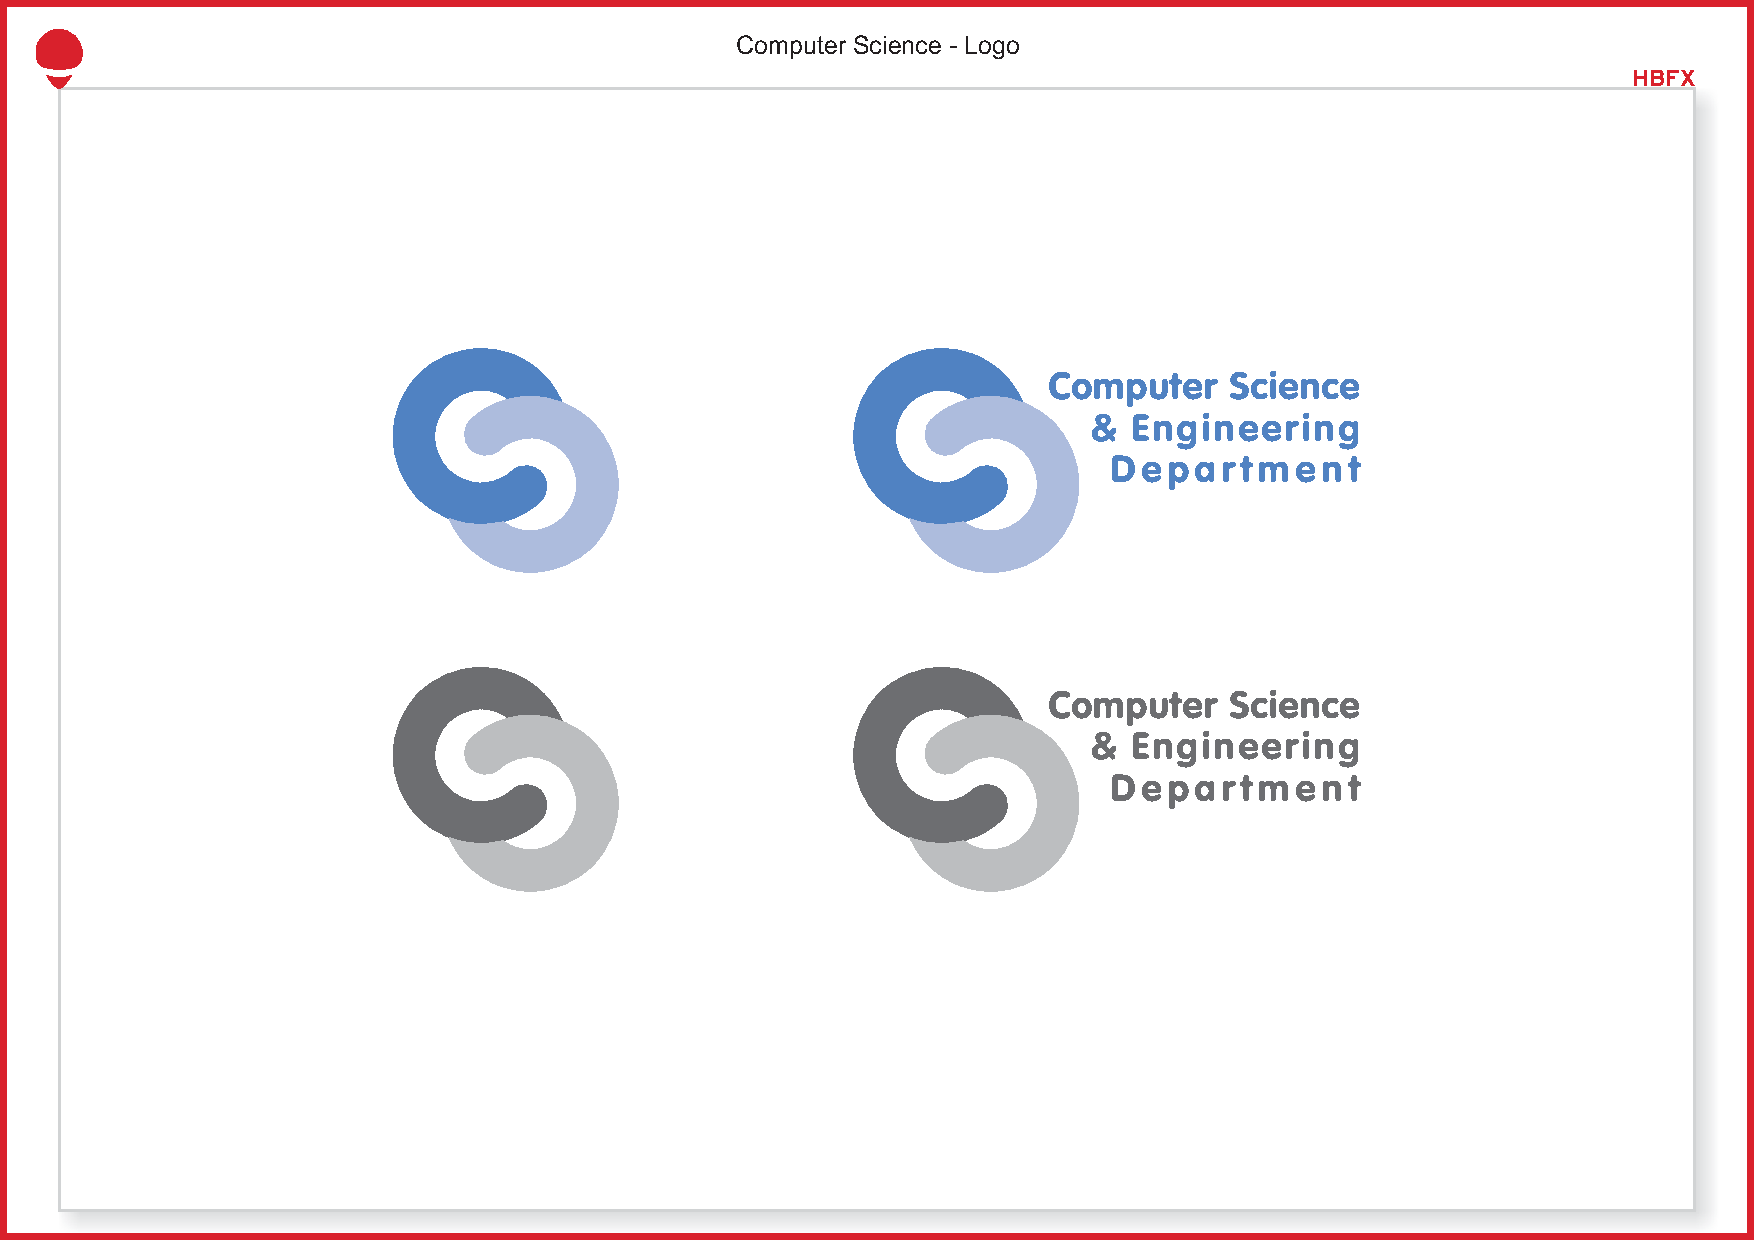
\includegraphics[scale=0.5,trim={14cm 11cm 2cm 5cm},clip=true]{pics/cs-logo.pdf}
\end{tabular}

\vspace{105pt}
{\Huge #2}\\                           % diploma project text
\vspace{40pt}
{\Large #3}\\ \vspace{0pt}  % project title
{\Large #4}\\                          % project subtitle
\vspace{40pt}
{\LARGE \Name}\\                   % student name
\end{center}
\vspace{60pt}
\begin{tabular*}{\textwidth}{@{\extracolsep{\fill}}p{6cm}r}
&{\large\textbf{#5}}\vspace{10pt}\\      % scientific advisor
&{\large \Advisor}                                    % advisor name
\end{tabular*}
\vspace{20pt}
\begin{center}
{\large\textbf{#6}}\\                                % bucharest
\vspace{0pt}
{\normalsize \Year}
\end{center}
\end{titlepage}
}

\newcommand{\frontPageRO}{\frontPage{\UniTextRO}{\DiplomaRO}{\ProjectTitleRO}{\ProjectSubtitleRO}{\AdvisorRO}{\BucRO}}
\newcommand{\frontPageEN}{\frontPage{\UniTextEN}{\DiplomaEN}{\ProjectTitleEN}{\ProjectSubtitleEN}{\AdvisorEN}{\BucEN}}

\linespread{1.15}
\setlength\parindent{0pt}
\setlength\parskip{.28cm}

%% Abstract macro
\newcommand{\AbstractPage}{
\begin{titlepage}
\textbf{\large SINOPSIS}\par
\AbstractRO\par\vfill
\textbf{\large ABSTRACT}\par
\AbstractEN \vfill
\end{titlepage}
}

%% Thank you macro
\newcommand{\ThanksPage}{
\begin{titlepage}
{\noindent \large\textbf{MULȚUMIRI}}\\
\Thanks
\end{titlepage}
}

%%%%%%%%%%%%%%%%%%%%%%%%%%%%%%%%%%%%%%%%%%%%%%%%%%   
%%
%%          End of template definitions
%%   
%%%%%%%%%%%%%%%%%%%%%%%%%%%%%%%%%%%%%%%%%%%%%%%%%%

\newcommand{\worktype}[1]{[\textit{#1}] }
\newcommand{\dezvoltare}{\worktype{Dezvoltare de produs}}
\newcommand{\cercetare}{\worktype{Cercetare}}
\newcommand{\ambele}{\worktype{Ambele}}

%%
%%   Campurile de mai jos trebuie modificate de autor. Modificati doar continutul, nu si numele fiecarei definitii
%%
\newcommand{\ProjectTitleRO}{Portarea unui sistem de operare pentru microprocesoare pe o platformă WebAssembly}
\newcommand{\ProjectTitleEN}{Porting an Embedded Operating System on WebAssembly}
\newcommand{\Name}{Niță Irina-Cristina}
\newcommand{\Advisor}{Prof. dr. ing. Răzvan Victor Rughiniș}
\newcommand{\Year}{2024}

% Setări document
\title{Proiect de diplomă}
\author{\Name}
\date{\Year}

%%
%%   Campurile aferente rezumatului
%%
\newcommand{\AbstractRO}{Sinopsisul proiectului are rol de introducere, conținând atât o descriere pe scurt a problemei abordate cât și o enumerare sumară a rezultatelor și a concluziilor. Se recomandă ca sinopsisul să fie redactat într-un limbaj accesibil unei persoane nefamiliarizate cu domeniul, dar în același timp destul de specific pentru a oferi rapid o vedere de ansamblu asupra proiectului prezentat.
Sinopsisul proiectului va fi redactat atât în română cât și în engleză. Ca dimensiunea recomandată aceasta secțiune va avea maxim 200 de cuvinte pentru fiecare variantă. Împreună, ambele variante se vor încadra într-o singură pagină.}

\newcommand{\AbstractEN}{The abstract has an introductory role and should engulf both a brief description of the issue at hand, as well as an overview of the obtained results and conclusions. The abstract should be formulated such that even somebody that is unfamiliar with the projects’ domain can grasp the objectives of the thesis while, at the same time, retaining a specificity level offering a bird’s eye view of the project.
The projects’ abstract will be elaborated in both Romanian and English. The recommended size for this section is limited to 200 words for each version. Together, both versions will fit in one page.}

%%
%%   Campurile aferente paginii de multumiri
%%
\newcommand{\Thanks}{(opțional) Aici puteți introduce o secțiunea specială de mulțumiri / acknowledgments. }

\begin{document}

\frontPageRO
\frontPageEN

\begingroup
\linespread{1}
\tableofcontents
\endgroup

\AbstractPage

% poate fi comentata sau stearsa
\ThanksPage

\selectlanguage{english}
\chapter{Introduction}\pagestyle{fancy}
This chapter...
\section{Context}

% WASM: Keywords: Viable, Sandbox, Platform Independent, Portable, Ubiquitous
% TockOS: Keywords: Embedded, Rust, Hybrid in terms of kernel
As microcontrollers (MCUs) are increasingly becoming more advanced,
embedded software developers have the ability to leverage the hardware to build
real-time systems that can run multiple applications simultaneously.
Coordinating multiple tasks on a platform with limited resources, such as memory,
implies running a memory-efficient operating system with, at least, a scheduler.
Due to good performance and low memory footprint, most systems are written in low-level
languages, usually C/C++, but are prone to memory-related security vulnerabilities.

Tock is an operating system written in Rust, a low-level systems programming language similar to C, but memory-safe.
As illustrated in \autoref{fig:tock},
the Rust feature seen most prominently in the Tock codebase is the separation between
safe and unsafe code. The operating system kernel and microcontroller-specific peripheral drivers
are considered "trusted" code, i.e. unsafe Rust is allowed; the drivers that define the application
program interfaces (APIs) for user applications are deemed "untrusted", i.e. unsafe Rust is forbidden.

% TODO: Image of Tock here

\begin{figure}[H]
\centering
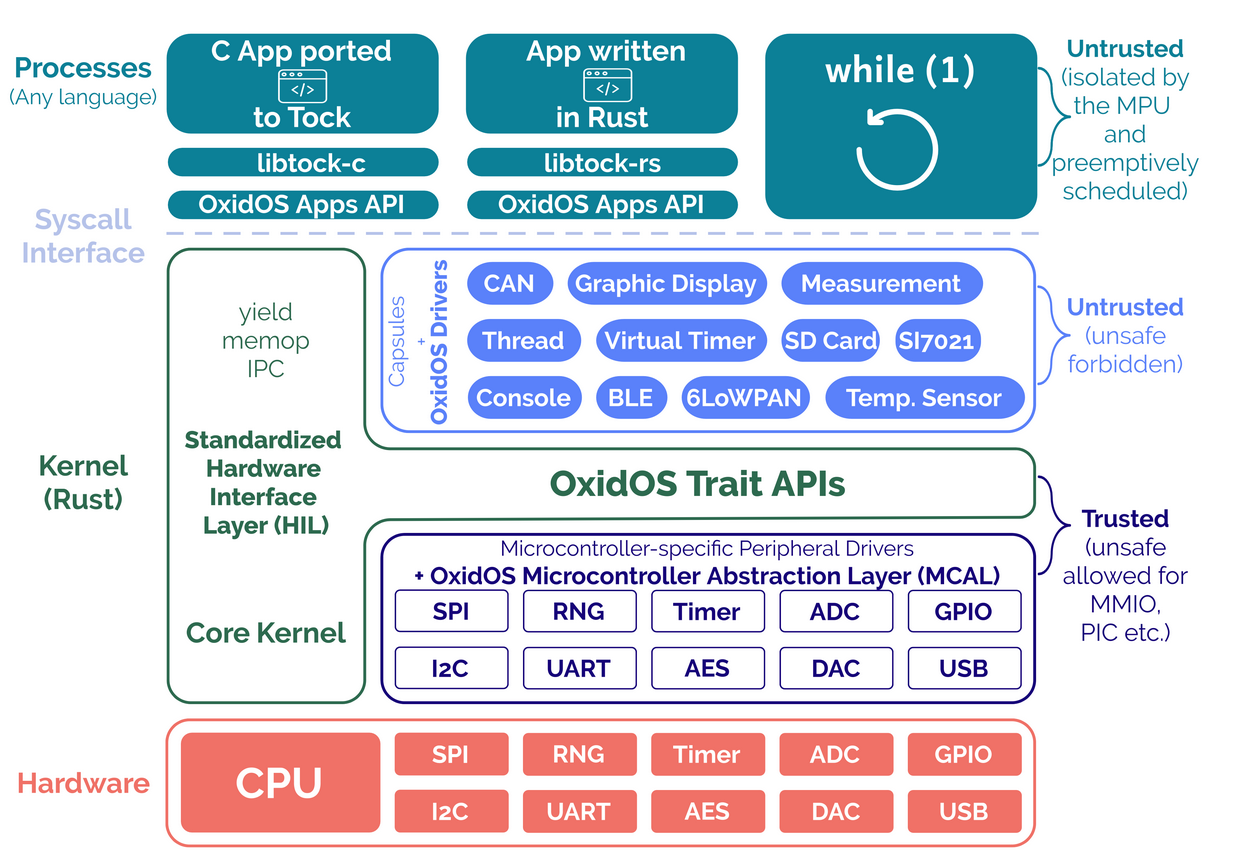
\includegraphics[scale=0.65]{pics/oxidos-stack.png}
  \caption[Tock operating system software stack]{Tock operating system software stack}
  \label{fig:tock}
\end{figure}

The abstraction acquired in Tock through Rust generics and traits (similar to "interfaces"
in other languages) ensures portability, allowing the drivers and kernel implementation to
remain agnostic regarding the hardware platform they are running on. Therefore, Tock could
eventually run on most targets if the minimum set of requirements for booting up the
kernel on a platform is met. The support list, alongside the modern MCUs' most prevalent
architectures (e.g. RISC-V, ARM), could include a more unusual choice, WebAssembly
(Wasm).

% TODO: Image of Wasm here
\begin{figure}[H]
\centering
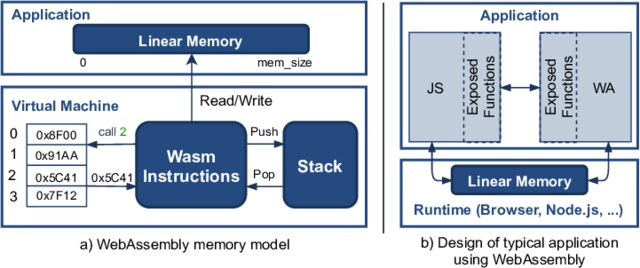
\includegraphics[scale=1.65]{pics/WebAssembly-high-level-architecture_W640-2.jpg}
  \caption[WebAssembly high-level architecture]{WebAssembly high-level architecture}
  \label{fig:wasm}
\end{figure}

WebAssembly is a binary instruction format that emerged from the Web's demand for interoperability with other programming languages, with the same or increased speed performance as native JavaScript. Through the portability of the Wasm compilation target, code written in low-level languages (C, C++ or Rust) is able to run on any platform, either Web embedded (in browser, e.g. Mozilla, or a JavaScript virtual machine, e.g. node.js) or in a non-Web environment (custom WebAssembly runtimes, e.g. Wasmtime). So, building Wasm support for an operating system inherently can be translated to building multi-platform support at once.

% TODO: Unicorn (that is also wasm)

\section{Motivation and Problem Statement} 

The main goal of this thesis is to provide a virtual environment for Tock by running the operating system on a transparent platform. The system is currently supported on Cortex-M and RISC-V chips; thus, it can only be tested on a physical board or an emulated one with significant restrictions. Adding support for WebAssembly eliminates the need for a hardware emulator (e.g., Qemu) during the software development process.

Part of Tock's porting process on Wasm consists of handling user applications through loading process binaries and handling system calls. Although the applications are not technically part of the operating system, Tock's virtualization process implies support for the whole environment, including user applications.

As of right now, the ability to run Tock locally is limited. The absence of physical hardware implies either using an architecture emulator, e.g., QEMU, which eliminates the idea of a simulation of peripherals, or third-party simulation software, e.g., WokWi, which is suitable for running a single embedded application on a well-known MCU but is restricted in terms of platforms it simulates and is not tailored to the operating system.

\section{Proposed Solution}

This thesis proposes an ecosystem incorporating support and tooling for developing Tock on users' machines, eliminating the necessity for physical hardware. The virtual platform comprises two components: the WebAssembly operating system kernel and the user applications that can be loaded into the platform's virtual flash memory.

The platform provides a debugger stub for the simulated environment to imitate the developing process on physical MCUs. This stub supports stepping through code, adding breakpoints, and getting information about registers and internal variables' values.

In addition to UART or timers, the simulation of hardware peripherals can extend to graphical-based interaction through communication between the user interface and the peripherals' behavior description protocol.

Tock's process console, a small shell over serial communication (UART), is available by simulating hardware peripherals for more debugging support. Users can access it via a terminal emulator to inspect the kernel and control userspace processes.

\section{Thesis Structure}

This paper begins with the background chapter, bringing the discussion into a theoretical context by providing introductory information on the technologies and terminology further used in the thesis.

The following chapter defines the architecture design for the system components at a higher level, remaining agnostic in implementation to the fullest extent possible.

\chapter{Background}\pagestyle{fancy}

This chapter...

\section{Rust}

\section{Tock}

Tock is an embedded operating system for low-power microcontrollers written in Rust, an alternative to the other candidate low-level programming languages like C. The Tock kernel is modular and comprises abstraction layers through Rust traits. As previously defined, Tock separates software-defined privilege rings by trustfulness, where allowing unsafe code is deemed an "act of trust." In other words, the closer the layer to necessary bare-metal programming, e.g., modifying registers, the more "trusted" the module. From a higher-level perspective, the operating system incorporates four components: the hardware interface layer, the microcontroller abstraction layer, the core kernel and the capsules.

\subsection{Hardware Interface Layer (HIL)}

TODO..

\subsection{Microcontroller Abstraction Layer (MCAL)}

TODO..

\subsection{Capsules}

TODO..

...

...

\section{WebAssembly and Deno}

WebAssembly is a binary format that ...

\section{Unicorn.js}

Unicorn Engine is a lightweight CPU emulator framework based on QEMU. The core is written in pure C and supports multiple binding languages. One example is the Unicorn.js package for JavaScript, which was ported through WebAssembly.

The emulator API allows users to modify registers, allocate memory for the virtual CPU, or define hooks for specific instructions or events.

\section{Remote GDB}

Due to resource limitation on embedded systems, the debugging process is usually done remotely. The process includes a very lightweight stub written on the chip and a debugger server running on the MCU. This thesis will reference GDB as the debugger,
but the LLDB protocol is very similar. (ref here)

% TODO diagrama aici plmm

\chapter{System Design and Architecture}

This chapter elaborates on the platform's design and architecture...

\section{WebAssembly kernel}

In order to simulate a physical MCU, the virtual microcontroller must have defined platform-specific peripherals. Currently, the simulator chip implements the functionality of four peripherals: timer, UART, GPIO, and CAN, which can be separated into two types of virtual peripherals:
the ones that can be dispatched to the user's system (timer, UART) and those that require simulation due to specific behaviors not directly found on one's local machine (GPIO, CAN). These peripherals must be configured and behave similarly to physical ones, regardless of their type.

% image here
[IMAGE HERE]

The next part of this section will discuss the design for the second type of peripheral in more depth because, as illustrated in [1], the first type's design is considered straightforward.

\section{Hardware-emulated userland processes and debugger}

The userland applications are compiled to a Cortex-M4 target and run using a hardware emulator. Due to the operating system running in a Wasm virtual machine in a non-emulated environment, a context switch between the kernel and the user processes implies updating the context for the emulated MCU.

Tock's context switch implementations are defined (separately from the microcontroller abstraction layer) for each supported architecture, being primarily written in inline assembly.

The remote debugger used for the hardware emulated user applications is implemented accordingly to the remote GDB specifications.

The stub server is running concurrently with the thread that runs the application, and share the
same information about the MCU's state.

\chapter{Implementation details}

This chapter...

\section{Microcontroller support for virtual platform}

\section{Deno virtual board}

\section{Unicorn.js hardware-emulated user processes}

\section{Context switch}

\chapter{Evaluation}

\chapter{Conclusions}

\chapter*{Bibliography}\addcontentsline{toc}{chapter}{Bibliography}  
% * <marios.choudary@gmail.com> 2018-02-28T12:07:48.730Z:
% 
% > BIBLIOGRAFIE
% Am adaugat un paragraf cu cateva detalii despre folosirea citarilor bibliografice in Latex, despre folosirea lui "\cite" si despre posibilitatea folosirii bibliografiei si direct in fisierul Latex.
% 
% ^.

\begin{itemize}
	\item 	NU utilizați referințe la Wikipedia sau alte surse fără autor asumat.
	\item 	Pentru referințe la articole relevante accesibile în web (descrise prin URL) se va nota la bibliografie și data accesării.
	\item 	Mai multe detalii despre citarea referințelor din internet se pot regăsi la:
	\begin{itemize}
		\item	\url{http://www.writinghelp-central.com/apa-citation-internet.html}
		\item	\url{http://www.webliminal.com/search/search-web13.html}
	\end{itemize}
	\item 	Note de subsol se utilizează dacă referiți un link mai puțin semnificativ o singură dată; Dacă nota este citată de mai multe ori, atunci utilizați o referință bibliografică.
	\item 	Dacă o imagine este introdusă în text și nu este realizată de către autorul lucrării, trebuie citată sursa ei (ca notă de subsol sau referință - este de preferat utilizarea unei note de subsol).
	\item 	Referințele se pun direct legate de text (de exemplu ``KVM [1] uses'', ``as stated by Popescu and Ionescu [12]'', etc.). Nu este recomandat să folosiți formulări de tipul ``[1] uses'', ``as stated in [12]'', ``as described in [11]'' etc..
	\item 	Afirmațiile de forma ``are numerous'', ``have grown exponentially'', ``are among the most used'', ``are an important topic'' trebuie să fie acoperite cu citări, date concrete si analize comparative.
	\begin{itemize}
		\item	Mai ales în capitolele de introducere, ``state of the art'', ``related work'' sau ``background'' trebuie să vă argumentați afirmațiile prin citări. Fiți autocritici și gândiți-vă dacă afirmațiile au nevoie de citări, chiar și cele pe care le considerați evidente.
		\item	Cea mai mare parte dintre citări vor fi în capitolele de introducere ``state of the art'', ``related work'' sau ``background''.
	\end{itemize}
	\item 	Toate intrările bibliografice trebuie citate în text. Nu le adăugați pur și simplu la final.
	\item 	Nu copiați sau traduceți niciodată din surse de informație de orice tip (online, offline, cărți, etc.). Dacă totuși doriți să oferiți, prin excepție, un citat celebru - de maxim 1 frază- utilizați ghilimele și evident menționați sursa. .
	\item 	Dacă reformulați idei sau creați un paragraf rezumat al unor idei folosind cuvintele voastre, precizați cu citare (referință bibliografică) sau cu notă de subsol sursa sau sursele de unde ați preluat ideile.
\end{itemize}

Trebuie respectat un singur standard de trimiteri bibliografice (citare), dintre următoarele alternative:
\begin{itemize}
	\item APA (\url{http://pitt.libguides.com/c.php?g=12108\&p=64730})
	\item IEEE (\url{https://ieee-dataport.org/sites/default/files/analysis/27/IEEE\%20Citation\%20Guidelines.pdf}) 
	\item Harvard (\url{https://libweb.anglia.ac.uk/referencing/harvard.htm})
	\item Cu numerotarea referințelor în ordine alfabetică sau în ordinea apariției în text (de exemplu, stilul cu numere folosit de unele publicații ACM - \url{https://www.acm.org/publications/authors/reference-formatting}) 
\end{itemize}

În Latex este foarte ușor să folosiți referințe într-un mod corect și unitar, fie prin adăugarea unei secțiuni
\verb!\begin{thebibliography}!
(vezi la sfârșitul acestei secțiuni), fie printr-un fișier separat de tip bib, folosind comanda
\verb!\bibliography{}!,
așa cum procedăm mai jos prin folosirea fișierului ``bibliography.bib''. În orice caz, în Latex va trebui să folosiți comanda
\verb!\cite{}!
pentru a adăuga referințe, iar această comandă trebuie folosită direct în text, acolo unde vreți sa apară citația, ca în exemplele următoare:
\begin{itemize}
	\item Articol jurnal: ~\cite{article};
	\item Articol conferință:~\cite{proc};
	\item Carte: ~\cite{book};
	\item Weblink: ~\cite{silva};
\end{itemize}

\textbf{Important}: în această secțiune de obicei apar doar intrările bibliografice (adică doar listarea referințelor). Citarea lor prin comanda cite și explicații legate de ele trebuie facute în secțiunile anterioare. Citarea de mai sus a fost facută aici doar pentru exemplificare.

% Asa se specifica folosirea unui fisier cu referinte bibliografice:
\bibliographystyle{plain}
\bibliography{bibliography}

%% O alta varianta ar fi fost includerea de articole direct in acest fisier
%% in felul urmator:
%% \begin{thebibliography}{ABC}
%%
%% \bibitem{article}
%%  H. Baali, H. Djelouat, A. Amira and F. Bensaali,
%%  ``Empowering Technology Enabled Care Using IoT and Smart Devices:
%   A Review''. In: IEEE Sensors Journal, vol. 322 (10), pp. 891--921, 1905.
%%
%% (more \bibitem items here...)
%%
%% \end{thebibliography}

%% Daca vreti ca o sectiune sa inceapa pe o pagina noua, puteti forta acest lucru cu comanda "\newpage", ca mai jos:

%\newpage

\chapter*{Anexe}\addcontentsline{toc}{chapter}{Anexe}

Anexele sunt opționale.
Ce poate intra în anexe:
\begin{itemize}
\item	Exemplu de fișier de configurare sau compilare;
\item	Un tabel mai mare de o jumătate pagină;
\item	O figura mai mare mai mare de jumătate pagină;
\item	O secvență de cod sursa mai mare de jumătate pagină;
\item	Un set de capturi de ecran (``screenshot''-uri);
\item	Un exemplu de rulare a unor comenzi plus rezultatul (``output''-ul) acestora;
\item 	În anexe intră lucruri care ocupă mai mult de o pagină ce ar întrerupe firul natural de parcurgere al textului.
\end{itemize}

\begin{appendices}

\chapter{Extrase de cod} % Introduce o nouă anexă
\ldots


\end{appendices}
\end{document}
